\chapter{Introduction}
\label{introduction}
The fundamental mechanism of radar is to transmit a radio signal and listen for reflections to gain information about remote targets. Although the concept of radar was evident from the beginnings of electromagnetic theory, it was not until sufficient transmitter and receiver technology was developed around the time of World War II that practical radars came into use for remote detection of ships and aircraft \autocite{Sko01}. Following the war, radar use branched out from military applications into scientific and commercial fields. Radar is still used with remote targets like aircraft and satellites for detection, tracking, and imaging, but it is more commonly encountered as a tool in weather or in highway speed limit enforcement \autocite{MS14}. Less known are the applications that drive the development of radar today, including autonomous landing systems for aircraft, driver-less cars, and terrain mapping (both surface and underground) of the Earth and other planets \autocite{Jol09, MS12}. But of the many uses of radar, one is somewhat unique in its requirements: the study of ionospheric plasmas. These plasmas vary widely in size, density, and persistence, so their study has necessitated the development of transmission coding and signal processing techniques that are adaptable to a wide range of circumstances. Unfortunately, the current techniques produce inherent processing artifacts or are inflexible in their application, limiting our ability to learn more about some ionospheric plasmas \autocite{VLV08a}.

The goal of this thesis is to develop new methods for radar data analysis that enable flexible, high-resolution measurements of ionospheric plasma phenomena. The key to achieving this goal lies in leveraging the concept of sparsity; scenes typically observed by a radar have a simple representation relative to the space of possible signals, and this prior information can help to improve measurements and analysis. In the case of measurements, this thesis presents a waveform inversion technique for removing ambiguity and self-interference due to the transmitted signal. In the case of analysis, a clustering method is developed for automatically detecting and classifying related scattering events. For events with a single point scatterer, we simulate and analyze statistics of matched filter interpolation for estimating target range and range-rate with increased resolution. Though the ionosphere provides the motivation and application for this work, the research is primarily focused on techniques that are generally applicable to most radar scenarios, especially those with multiple or distributed scatterers.

The remainder of this chapter broadly covers the ionosphere, radar, and sparsity in order to motivate the research and set the stage for later developments. Section \ref{intro_ionosphere} gives background information on the ionosphere and describes its effects on radio communications, its role in studying the science of the geospace system, and its function in observing meteoroids that pose a threat to orbiting satellites. Section \ref{intro_radar} describes the radars used to study the ionosphere, the types of scattering that are typically encountered, and the challenges they present. Section \ref{intro_sparsity} details the function of sparsity in efficient information processing and its emerging role in many different fields of research. Finally, Section \ref{contributions} outlines the contributions of this dissertation, and Section \ref{outline} provides a reader's guide for the remaining chapters.

\section{The Ionosphere}
\label{intro_ionosphere}
Surrounding the Earth is a region defined by ionization: the ionosphere. It is a portion of the upper atmosphere where charged particles, both electrons and ions, are present in addition to neutral air molecules. This region extends from approximately 60 km to 2000 km in altitude, a range which includes the low Earth orbits (LEO) inhabited by the majority of satellites. The ionized and neutral particles constitute a plasma, one that varies greatly over time and over the spatial extent of the ionosphere. Driving these variabilities are interactions with the lower atmosphere and the space environment, most notably radiation from the sun. As the interface between space and the Earth's atmosphere, the ionosphere is difficult to study but critically important for understanding the geospace system \autocite{CEDAR11}.

\subsection{Formation and Variability}
\label{intro_ionosphere_formation}
Ionization of neutral air molecules by solar radiation is the primary cause for the existence of the ionosphere, and it is balanced by ion-electron recombination chemistry. Recombination limits the maximum ionized plasma density during the day and dissipates the plasma at night. Naturally, the temporal peak in plasma density happens near noon when the ionization rate is at its highest, but even then the plasma density is at most around one percent of the neutral background. Example plasma densities for the daytime and nighttime mid-latitude ionosphere are shown in Figure \ref{fig:ionospheric_density}.
\begin{figure}[tpb]
 \centering
 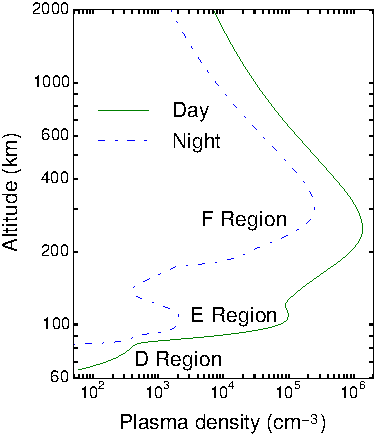
\includegraphics{ionospheric_density}
 \caption[Ionospheric plasma density during day and night]{\emph{Ionospheric plasma density during day and night.} This plot shows predicted electron density at noon and midnight on December 1, 2014, according to the IRI-2012 model \autocite{BAZ+14}. The prediction is for the mid-latitude ionosphere above the Millstone Hill incoherent scatter radar.}
 \label{fig:ionospheric_density}
\end{figure}%
Solar radiation ionizes air molecules down to altitudes of approximately 60 km, forming the ionosphere's lower boundary. Its upper boundary at approximately 2000 km altitude is more tenuously defined; it is not a cutoff of ionization but rather one of sufficient density to exhibit bulk plasma properties. Between these boundaries, the ionosphere is divided by altitude into different regions defined by variations in plasma density. Arranged by increasing altitude, these layers are called the D, E, and F regions. The different regions exist because the ionization rate varies with altitude: solar intensity decreases with decreasing altitude as more radiation is absorbed, while at the same time the neutral atmosphere increases in density and varies in composition with decreasing altitude due to gravity \autocite{Tas10, Kel09}.

Though this simple model is useful to conceptualize the ionosphere, it is important to note that the ionosphere is part of a complex geospace system and therefore exhibits significant variability over time and space. Day/night variability has already been mentioned, but tidal, seasonal, and solar activity cycles are also significant drivers of the ionosphere. Weather is an important contributor on shorter timescales, both in terms of atmospheric weather from the dynamics of the neutral atmosphere and space weather from the flares and particle precipitation of solar storms. In terms of spatial variability, the changing orientation of the Earth's magnetic field lines with respect to latitude divides ionospheric behavior into three regions: equatorial, polar, and mid-latitude. In the equatorial region, the magnetic field lines are horizontal. This results in unique plasma dynamics that include the equatorial electrojet current sheet, turbulence-induced field-aligned irregularities, and equatorial bubbles \autocite{Kel09}. In the polar region, the magnetic field lines connect to the magnetosphere and solar wind and bring a supplemental source of energetic particles. The result is enhanced ionization and light displays known as aurora, among other phenomena \autocite{KR95}. The mid-latitude region lies between the other two and is defined through the absence of equatorial and polar effects. Boundary interactions are characteristic of this region, including the plasmasphere boundary layer of the sub-auroral zone \autocite{CL04} and notable disturbances like sudden stratospheric warming \autocite{GHB+13}.

\subsection{Communications and Irregularities}
\label{intro_communications}
The ionosphere is felt most strongly in daily life through its effects on radio communications. Radio waves of lower frequency (less than about 13 MHz for a typical F-region peak plasma density \autocite{Tas10}) reflect off of the ionosphere. In practical terms, AM radio broadcasts reflect (when they are not absorbed), while the higher-frequency FM radio signals pass through the ionosphere into space. However, even the higher microwave-frequency signals that are typically used for satellite communications are subject to attenuation, refraction, and delay \autocite{Kel09}. This is especially important to consider in the case of the global navigation satellite systems (GPS, GLONASS, Galileo); these depend on precise timing and require correction for ionospheric effects in order to achieve high positioning accuracy.

Ionospheric irregularities are even more important to characterize, due to their unpredictability and potential to completely disrupt typical satellite communications. Random variation of signal strength and phase, termed scintillation, occurs whenever there are abrupt changes in electron density along the signal path. These irregularities cause scattering and self-interference of a radio signal, a process analogous to looking through rough glass. The result is corrupted communication or even loss of signal. Figure \ref{fig:scintillation} depicts the measured signal for a radar beam sweeping back and forth across a calibration target.
\begin{figure}[tpb]
 \centering
 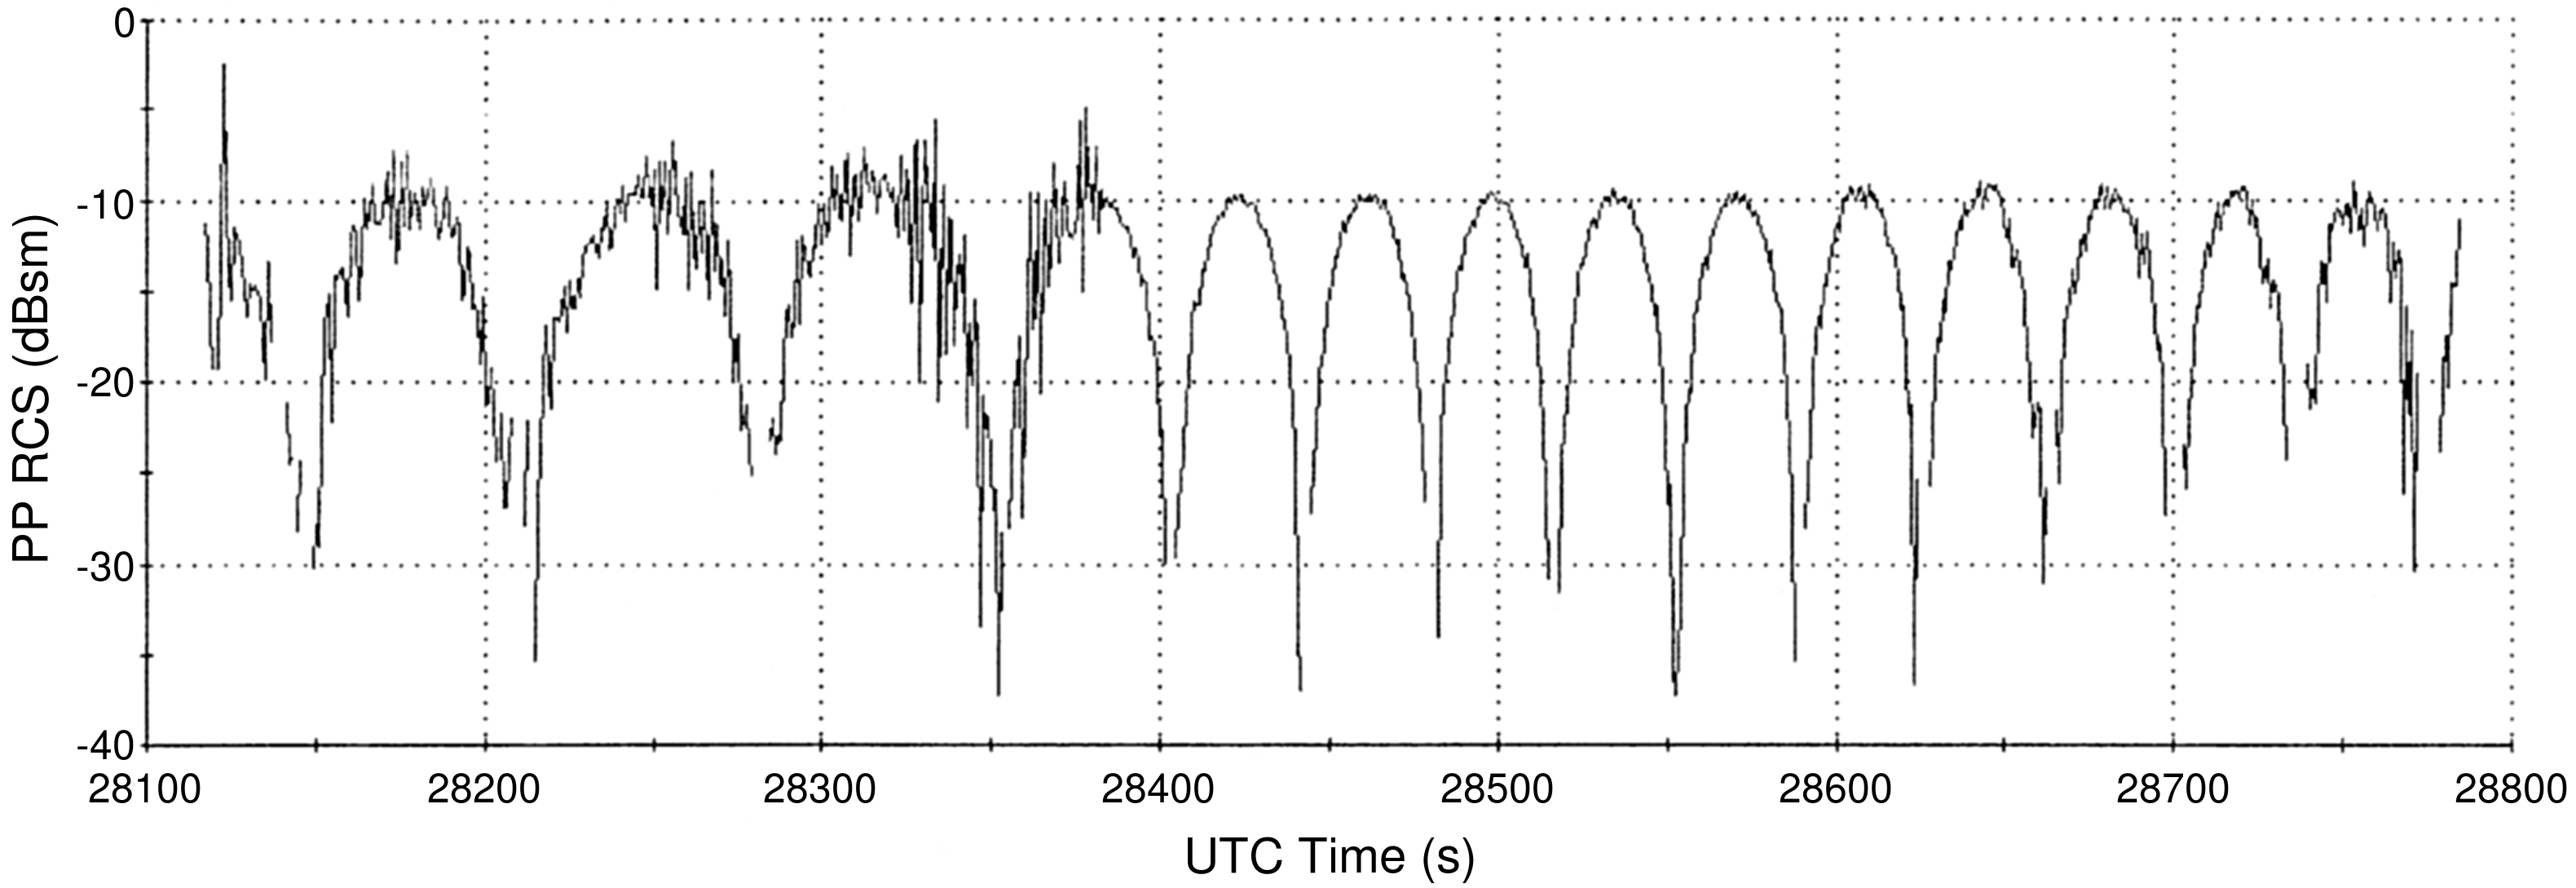
\includegraphics{scintillation}
 \caption[Scintillation of a radar calibration signal]{\emph{Scintillation of a radar calibration signal.} This plot shows the radar cross section (RCS) measured for the principal polarization (PP) from a calibration test with the ALTAIR radar at 160 MHz. The radar beam was swept back and forth across a fixed target, so the signal strength is expected to be consistent with each pass. Scintillation is evident on the first four and a half passes, while the rest are nearly scintillation-free.}
 \label{fig:scintillation}
\end{figure}%
The first four passes exhibit scintillation as strong variations in signal strength, while the remaining passes are nearly scintillation-free. Though categorized as an irregularity, scintillation is an everyday occurrence arising from typical variation of the ionosphere. Geomagnetic storms, in contrast, are truly irregular occurrences arising from solar activity. They disrupt the ionosphere by increasing direct energy input and transport effects, thus triggering further irregularities and scintillation \autocite{Kel09}.

\subsection{System Science}
\label{intro_system_science}
Given how much the world depends on satellite communications and radio systems, studying the ionosphere in order to predict and mitigate disruptions is clearly important. In order to do that, though, it is necessary to examine the ionosphere's role in the overall geospace system. This system is formed of complex interactions between the Earth, with its atmosphere and magnetic field, and the space environment, with the dominating influence of the Sun. Scientific study of the geospace system in the past has been limited by the inability to investigate its complexity, eloquently described by the \textcite{CEDAR11} as the "many interacting elements that, as a whole, exhibit properties not obvious from the properties of the individual parts." Nevertheless, this so-called systems science is becoming more feasible every day with the advancement of computational and measurement techniques. Since the ionosphere is a key cog in the geospace system, it is important to develop new methods for studying the ionosphere that embrace complexity and enable improved understanding of the system as a whole. This requires measurements that are universal, encompassing large portions of the ionosphere, and it requires techniques that are flexible, measuring plasmas spanning a wide range of size, density, and persistence.

\subsection{Meteoroids and Meteors}
\label{intro_meteoroids}
Of the many components of the space environment that interact with the ionosphere, meteoroids warrant special mention. \emph{Meteoroid} is a term that encapsulates any small, naturally occurring solid body in space. Meteoroids range in size from 10 micrometers to approximately 1 meter in diameter; smaller particles are called dust, and larger bodies are called asteroids \autocite{RG10}. While an asteroid crossing paths with the Earth is a rare event of global disaster proportions, meteoroids routinely enter the Earth's atmosphere. Furthermore, meteoroids are more common as size decreases; roughly speaking, their number are inversely proportional to the mass of the meteoroid squared as shown in Figure \ref{fig:meteoroid_mass_distribution}.
\begin{figure}[tpb]
 \centering
 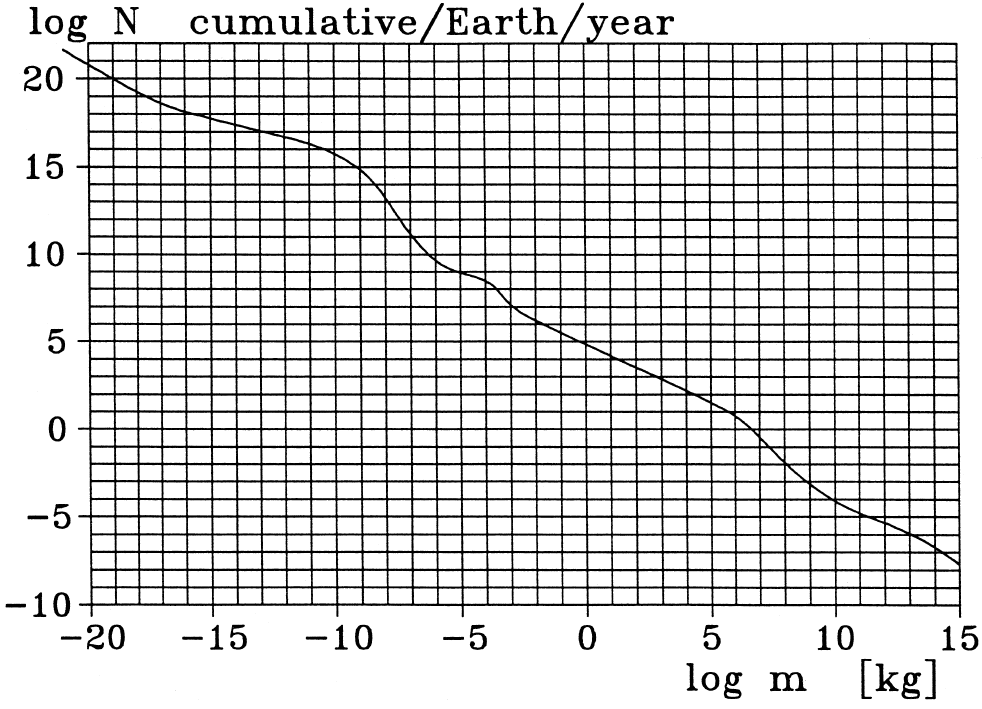
\includegraphics[width=0.6\textwidth]{ceplecha_meteoroid_count_vs_mass}
 \caption[Cumulative distribution of interplanetary bodies as a function of mass]{\emph{Cumulative distribution of interplanetary bodies as a function of mass.} This plot, reproduced from \textcite{CBE+98}, shows the cumulative count $N$ of interplanetary bodies (including meteoroids and asteroids) with mass greater or equal to $m$ that enter the Earth's atmosphere per year. Both the count and mass are plotted as base-10 logarithms.}
 \label{fig:meteoroid_mass_distribution}
\end{figure}%
As a point of reference, on the order of 100 million meteoroids big enough to be detected by high-power large aperture radars (0.1 micrograms or larger \autocite{CBC+07}) are estimated enter the Earth's atmosphere every second on average \autocite{CBE+98}; this is equivalent to approximately one meteoroid every second within a radar beam that is pointed upward with a one degree half-power beamwidth. If a meteoroid survives passage through the atmosphere and lands on the Earth, which is correspondingly more rare, the surviving body is called a \emph{meteorite}.

The term \emph{meteor} is not to be confused with meteoroid, although they are often incorrectly used interchangeably. A meteor denotes the plasma created by a meteoroid as it speeds through the atmosphere, typically forming between 80 and 120 km in altitude. Sometimes light is emitted when the meteoroid is large or fast enough, and this is also called a meteor or colloquially a shooting star. Meteoroids enter the atmosphere with such speed, typically between 11 and 72 km/s \autocite{CBE+98}, that they heat up, ablate their constituents, and cause some of the surrounding air to ionize. The resulting plasma is many times denser than the background ionospheric plasma, but it typically only retains that density for a fraction of a second before diffusing and recombining \autocite{Jon95, DWB+08}. The plasma dynamics spurred by meteors are significant to the overall ionospheric system, while the ablated meteoroid elements play an important role in the chemistry of the upper atmosphere.

Aside from their role in driving ionospheric processes, meteoroids are also important because of the likelihood that they will impact satellites. The most prevalent meteoroids are small enough ($<$ 1 microgram) that they can't do physical damage; however, meteoroids travel fast enough that even the smaller ones can cause electrical damage to satellites through the plasma that they create upon impact \autocite{CCC+10}. \textcite{LCG+13} showed through ground experiments that this damage is possible and could explain nebulously-attributed or otherwise unexplained anomalies and failures of a number of satellites. In order to better characterize the electrical threat to satellites, we need better methods of remotely measuring the meteoroid distributions of rate, size, speed, and composition; the best way to do that is by advancing radar techniques for observing meteors.

\section{Radar Measurements}
\label{intro_radar}
Due to its remoteness and size, spanning altitudes from 60 km to 2000 km, the ionosphere is difficult to study. Even the lowest reaches of the ionosphere are outside the range of aircraft, leaving balloons, rockets, and satellites as the only carriers for \emph{in situ} measurement equipment. Not only are these methods expensive, but they also do not give enough data over time and space to perform more than localized studies. For large-scale observation of the ionosphere, scientists are left with methods of remote sensing, particularly radar.

\subsection{Incoherent Scatter Radars}
\label{intro_isrs}
It takes a large radar to be sensitive enough to measure scattering from electrons in the background ionosphere; this type of signal is called incoherent scatter, and these large radars are incoherent scatter radars (ISRs) \autocite{Gor58}. There are only about a dozen ISRs in operation across the globe, with locations depicted in Figure \ref{fig:isr_map}.
\begin{figure}[ptb]
 \centering
 \begin{subfigure}{\textwidth}
  \centering
  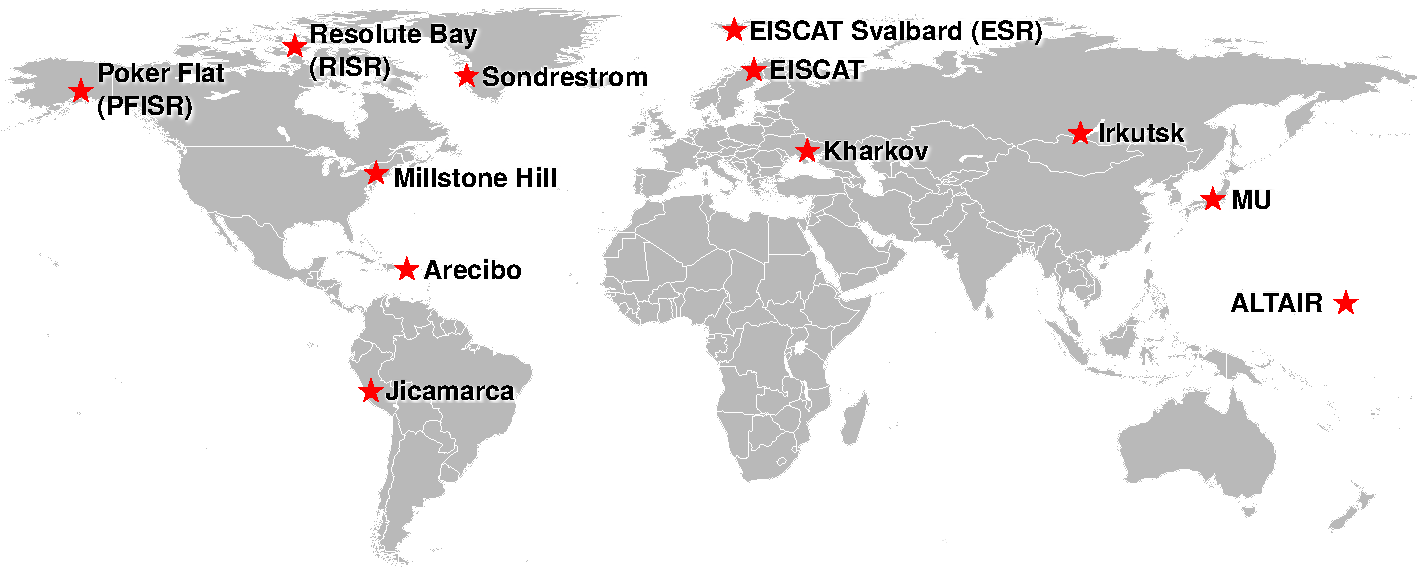
\includegraphics[width=0.9\textwidth]{isr_map}
  \caption{Map of Incoherent Scatter Radars (ISRs)}
  \label{fig:isr_map}
 \end{subfigure}
 \begin{minipage}[b]{0.49\textwidth}
 \begin{subfigure}[b]{\textwidth}
  \centering
  \includegraphics[width=\textwidth,trim=0px 20px 0px 105px,clip]{jicamarca}
  \caption{Jicamarca ISR}
  \label{fig:jicamarca}
 \end{subfigure}
 \begin{subfigure}[b]{\textwidth}
  \centering
  \includegraphics[width=\textwidth]{pfisr}
  \caption{Poker Flat ISR (PFISR)}
  \label{fig:pfisr}
 \end{subfigure}
 \end{minipage}
 \begin{subfigure}[b]{0.49\textwidth}
  \centering
  \includegraphics[width=\textwidth]{millstone_hill_radar}
  \caption{Millstone Hill ISR}
  \label{fig:millstone}
 \end{subfigure}
 \caption[Incoherent scatter radars spanning the globe]{\emph{Incoherent scatter radars spanning the globe.} Locations of the current ISRs are shown in \textbf{(\subref{fig:isr_map})}. The Jicamarca ISR \textbf{(\subref{fig:jicamarca})} is a phased array of dipole antennas located outside of Lima, Peru. The Poker Flat ISR \textbf{(\subref{fig:pfisr})} is a modern phased array located in Poker Flat, Alaska. The Millstone Hill ISR \textbf{(\subref{fig:millstone})} is composed of one steerable dish antenna and one fixed zenith dish antenna and is located outside of Boston, Massachusetts.}
 \label{fig:isrs}
\end{figure}%
Each radar covers a small slice of the ionosphere ranging from equatorial latitudes (e.g. Jicamarca outside Lima, Peru; Figure \ref{fig:jicamarca}) through mid-latitudes (e.g. Millstone Hill near Boston, MA; Figure \ref{fig:millstone}) to polar latitudes (e.g. the Poker Flat ISR in Alaska; Figure \ref{fig:pfisr}). The main parameters of the various ISRs are given in Table \ref{tab:isr_parameters}.
\begin{table}[tb]
 \renewcommand{\arraystretch}{1.2}
 \begin{center}
 \caption[Incoherent scatter radar parameters]{\emph{Incoherent scatter radar parameters.}}
 \label{tab:isr_parameters}
 \begin{tabular}{@{}llllll@{}} % @{} removes space from edge
  \toprule
  Radar & Frequency & Bandwidth & Peak Power & Gain & Size\\
  & (MHz) & (MHz) & (MW) & (dBi) & (m)\\
  \midrule
  ALTAIR\footnotemark[1] & 160/422 & 7/18 & 6 & 34/42 & 46\\
  Arecibo\footnotemark[2] & 430 & 1 & 2.5 & 62 & 305\\
  EISCAT VHF\footnotemark[3] & 224 & 1 & 1.6 & 46 & 120 $\times$ 40\\
  EISCAT UHF\footnotemark[3] & 931 & 1 & 2 & 48.1 & 32\\
  ESR\footnotemark[3] & 500 & 1 & 1 & 42.5/45 & 32/42\\
  Irkutsk\footnotemark[4] & 154 & 0.014 & 3.2 & 35 &\\
  Jicamarca\footnotemark[5] & 50 & 1 & 4.5 & 42.6 & 300 $\times$ 300\\
  Kharkov\footnotemark[6] & 158 & 0.015 & 2 & 40 & 100\\
  Millstone\footnotemark[7] & 440 & 1 & 2.5 & 42.5/45.5 & 46/68\\
  MU\footnotemark[8] & 46.5 & 1.65 & 1 & 34 & 103\\
  PFISR\footnotemark[9] & 450 & 1 & 2 & 43 & 30 $\times$ 30\\
  RISR\footnotemark[10] & 442.5 & 1 & 2 & 43 & 30 $\times$ 30\\
  Sondrestrom\footnotemark[11] & 1290 & 1 & 3 & 50 & 32\\
  \bottomrule
 \end{tabular}
 \end{center}
 
 \footnotesize
 [\footnotemark[1]\cite{TBOT79}; \footnotemark[1]\cite{CHMM02}; \footnotemark[2]\cite{Hag05}; \footnotemark[3]\cite{EISCAT_SPEC}; \footnotemark[4]\cite{PMZ+08}; \footnotemark[5]\cite{Och63}; \footnotemark[5]\cite{JICAMARCA_SPEC}; \footnotemark[6]\cite{BTC06}; \footnotemark[7]\cite{Eva65}; \footnotemark[7]\cite{MILLSTONE_SPEC}; \footnotemark[8]\cite{FST+85}; \footnotemark[9]\cite{CGHN09}; \footnotemark[9]$^{,}$\footnotemark[10]\cite{AMISR_SPEC}; \footnotemark[11]\cite{KHVV95}]
\end{table}%
Most of their characteristics are roughly similar, with megawatt-class transmitters, high gain, and large size. The baseband frequencies are all in the VHF and UHF bands, greater than 30 MHz and less than 3 GHz, which places them above the ionosphere's peak plasma frequency and allows the electromagnetic waves to completely penetrate the plasma. The ISRs also come in one of two broad forms, with either focusing reflector dishes like Millstone Hill or distributed antenna arrays like Jicamarca and the Poker Flat ISR (PFISR). The dish radars are usually mechanically steerable which limits their view to one region of the sky within a short period of time, while the array radars are electronically steerable which allows the location of their electromagnetic sensitivity to be adjusted by changing the phase of the antenna connections. At older arrays like Jicamarca, this phasing is still done mechanically by hand, while newer arrays like PFISR are phased by computer control and so can look at completely different portions of the sky from pulse to pulse \autocite{Och63, CGHN09}.

\subsection{Examples of Ionospheric Radar Scatter}
\label{intro_radar_scatter_examples}
In addition to the background ionospheric plasma, ISRs are also used to measure other plasma processes and irregularities which exhibit stronger signals. This thesis heavily utilizes data taken with the Jicamarca ISR, and one of the processes that is frequently encountered there is the equatorial electrojet. The electrojet arises from the unique geometry of the magnetic equator, where the magnetic field is parallel to the Earth's surface. This geometry, coupled with the existing east-west zonal current from E-region winds, creates a vertical electric field that greatly enhances the zonal current through $E \times B$ drift to form the electrojet \autocite{Kel09}. When the current of the electrojet is strong enough, it produces plasma density irregularities that coherently scatter a radar signal at many orders of magnitude greater than the strength of incoherent scatter. As shown in Figure \ref{fig:electrojet_example}, electrojet scatter is compact in range and resides near an altitude of 100 km.
\begin{figure}[tbp]
 \centering
 \begin{tikzpicture}[very thick]
  \node[above right,image] at (0,0) {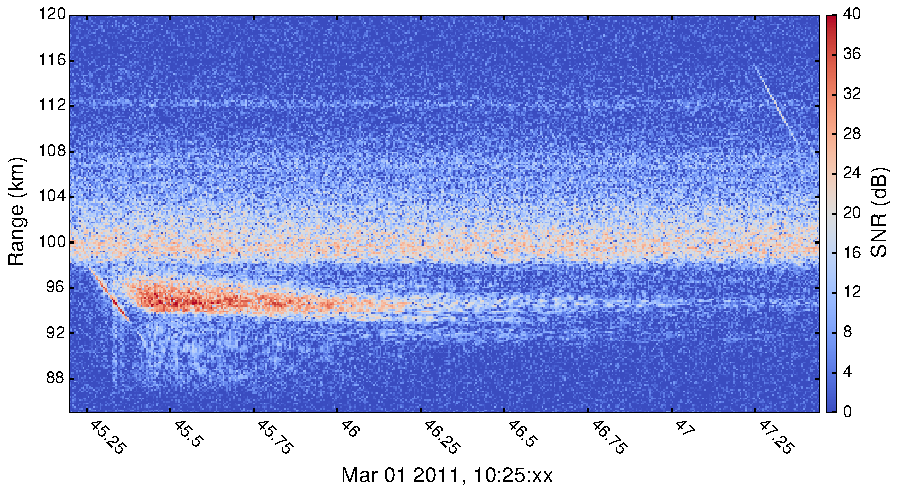
\includegraphics{equatorial_example_mf_rti_3}};
  \draw[green!80!black] (1.15,3.93) rectangle (13.95,4.74);
  \draw[purple] (1.4,2.8) rectangle (11.5,3.87);
  \draw[purple] (12.6,5.8) rectangle (13.7,7.4);
 \end{tikzpicture}
 \caption[The equatorial ionosphere as measured by the Jicamarca ISR]{\emph{The equatorial ionosphere as measured by the Jicamarca ISR.} Scattering due to the \textcolor{green!80!black}{equatorial electrojet} is seen in a narrow band around 100 km range (altitude). The other significant scattering is due to two \textcolor{purple}{meteors}.}
 \label{fig:electrojet_example}
\end{figure}%
It also is relatively stationary, and so it produces no Doppler frequency shift to complicate the scattered signal. Though the electrojet is important in its own right, it is often seen as clutter when trying to measure other ionospheric processes.

Another ubiquitous class of scatterers in the equatorial ionosphere and globally are meteors. When viewed by a high-power large-aperture (HPLA) radar like the ISRs, meteors exhibit two types of scattering: head echoes and trail echoes. Both are shown in Figure \ref{fig:meteor_scattering_example}.
\begin{figure}[tbp]
 \centering
 \begin{tikzpicture}[very thick]
  \node[above right] at (0,0) {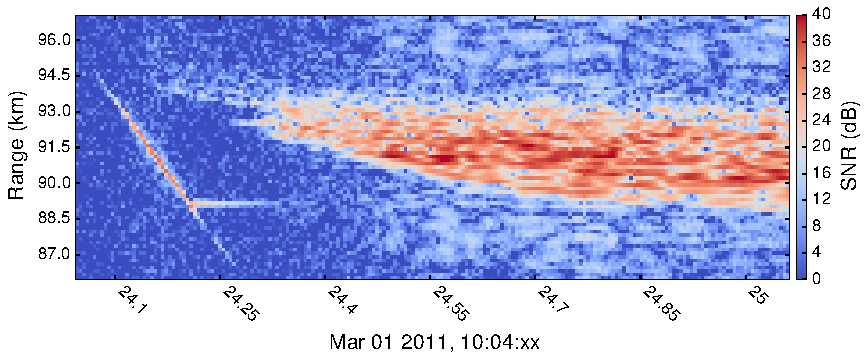
\includegraphics{head_and_flare_mf_rti_3}};
  \draw[purple] (2.7,5) -- (2.7,4.5) -- (8.5,2.6) -- (13.575,2.6) -- (13.575,5) -- cycle;
  \draw[green!80!black,shift={(2.9,3.5)},rotate=-55] (-2.15,-0.235) rectangle (2.15,0.235);
  \draw[yellow!80!black] (3.3,2.65) rectangle (5,3);
 \end{tikzpicture}
 \caption[Examples of meteor head and trail echoes]{\emph{Examples of meteor head and trail echoes.} Two types of meteor scattering are observed from the same meteor by the Jicamarca ISR. The \textcolor{green!80!black}{head echo} is the narrow streak on the left, while the \textcolor{purple}{non-specular trail echo} is the range-spread scattering on the right. The head echo also exhibits a \textcolor{yellow!80!black}{flare} with a sudden increase in signal strength and longer-lasting scattering at about 89 km range (altitude).}
 \label{fig:meteor_scattering_example}
\end{figure}%
A head echo represents scattering from the dense ball of plasma traveling with the meteoroid \autocite{CODD05}. In a radar signal intensity image plotted as range (or altitude) versus time (known as a range-time-intensity or RTI plot), head echoes appear as a narrow streak that descends in altitude with time. Because the meteoroid and head plasma are moving at high speed toward the radar as they descend in altitude, head echoes have a large positive Doppler frequency shift that complicates their measurement. Observing the head echo's speed, either by change in altitude or through the Doppler shift, allows one to determine the meteoroid's speed. If angular speed measurements are available through interferometry or monopulse, the full velocity and hence orbit of the meteoroid can be calculated. In addition, the signal strength and deceleration of the head echo can be used to determine the mass and density of the parent meteoroid \autocite{CVL+12}.

Once the meteor plasma is created by the meteoroid, it diffuses quickly into a trail that is left behind in the meteoroid's wake. Scattering from the trail can then happen either specularly or non-specularly. For specular scattering, the line of trail plasma acts like a mirror to reflect the radar signal \autocite{Sug64}; with a monostatic radar system where the transmitting and receiving antenna are one in the same, this means that the meteor trail must be perpendicular to the radar pointing direction in order for it to be seen specularly. Non-specular scattering is only possible when the radar points near perpendicularly to the Earth's magnetic field; turbulence sets up field-aligned irregularities of the trail plasma within a few tenths of seconds, providing enhanced scattering in the direction perpendicular to the magnetic field until the irregularities dissipate after a few seconds \autocite{DOCH02}. The example seen in Figure \ref{fig:meteor_scattering_example} is of a non-specular trail. Both types of trail echoes can be used to calculate meteoroid speed \autocite{CES97, DDC+04} and observe upper atmospheric winds \autocite{HFV01, OSS+09}.

\subsection{Challenges}
\label{intro_radar_challenges}
Much of what we know about the ionosphere has been gleaned from radar data, but there are still processes that are difficult to analyze. Radar presents an inherent conflict between sensitivity and ambiguity; longer transmitter pulses are needed to put more energy on target, but they have a correspondingly poorer range discrimination capability. Pulse compression, encoding the waveform on transmission and decoding the returned signal on reception using matched filtering, is the standard way to settle the conflict. However, matched filtering still results in ambiguity in the form of self-clutter \autocite{Woo80}. Because of this conflict, it is difficult to make high quality measurements in situations where both sensitivity and high resolution are needed.

With meteors, for example, we lack good observations of two phenomena: fragmentation and flares. In the case of fragmentation, \textcite{MBMC10} show meteor head echoes with an oscillating signal intensity that they explain by modeling the signal as interference between two separate scattering centers, with the theory that such a signal represents the result of meteoroid fragmentation. An example of this oscillation is shown in Figure \ref{fig:mathews_fragmentation}, but the fragmentation theory that could explain it has not been definitively proven.
\begin{figure}[tbp]
 \centering
 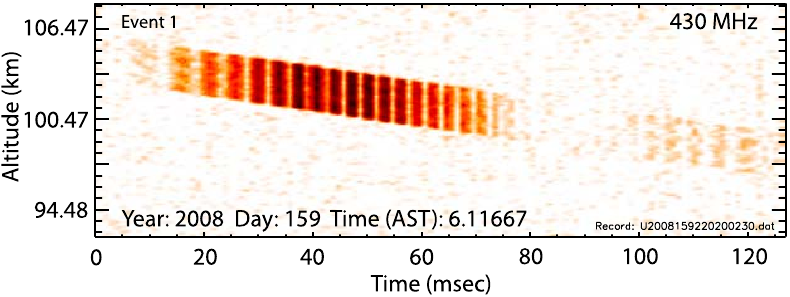
\includegraphics[width=0.75\textwidth]{mathews_fragmentation}
 \caption[Meteor head echo oscillations]{\emph{Meteor head echo oscillations.} This data from the Arecibo radar shows a meteor head echo with oscillating signal strength. The figure is reproduced from \textcite{MBMC10}, and unfortunately no color scale for the signal strength was given. \textcite{MBMC10} theorize that this oscillation indicates interference between two distinct head echo scatterers produced by meteoroid fragmentation.}
 \label{fig:mathews_fragmentation}
\end{figure}
Flares and the related terminal events are a process sometimes seen with head echoes where the signal intensity suddenly increases and trail scattering is immediately visible at the location of the event. An example of this process can be seen in Figure \ref{fig:meteor_scattering_example}, where a flare accompanies the meteor head echo. Currently no evidence has been observed that would explain why flares happen. Higher resolution data with reduced ambiguity is necessary to find answers to these mysteries, but such data cannot be produced with current techniques.

These challenges are somewhat unique to the applications found in the ionospheric radar community. Because of the wide variety of plasma processes and the corresponding demands on detail in space, time, and frequency, a wide variety of transmission waveforms are used. Some of these waveforms use deliberately-spread energy in frequency space to break the inherent relationship between sensitivity and resolution. Unfortunately, matched filter processing brings ambiguity and decoding artifacts, problems which cannot be ignored due to the high range of signal strength from one scatterer to the next. Current radar measurement techniques need to improve in four major areas to meet the challenges presented by the host of ionospheric plasma processes:
\begin{inparaenum}[1)]
 \item Differentiation of targets in crowded and variable environments, such as the ability to separate meteor and electrojet signals in the equatorial ionosphere;
 \item Elimination of self-interference of range-spread targets, which include non-specular meteor trails among others;
 \item Higher resolution to observe small-scale processes, such as meteoroid fragmentation and meteor flares; and
 \item Flexibility to achieve all of these goals at once.
\end{inparaenum}

\section{Sparsity}
\label{intro_sparsity}
The concept of sparsity is fundamental to how the brain processes information and manages to make sense of the deluge of sensory inputs that it receives. This principle, known as \emph{sparse coding}, states that "information is represented [in the brain] by a relatively small number of simultaneously active neurons out of a large population" \autocite{OF04}. Sparse coding makes the inherent structure of natural signals explicit, providing increased storage capacity and better energy efficiency in addition to simplifying higher-level reasoning. To achieve sparse coding, individual neurons respond to and represent just one particular aspect of a sensory input: an image is viewed through the retina, and a small number of neurons in the visual cortex respond to the image's localized patterns and edges \autocite{OF97}; a sound resonates at the individual frequencies of the inner ear hairs, and a sparse collection of neurons respond to the different frequency bands and corresponding time windows of the wave \autocite{Lew02}. The responses of the individual neurons collectively form a dictionary from which a small number of elements are used to represent any one particular input. Though this neurological example represents just one case of the practical use of sparsity, the concept of finding simple descriptions to represent and reason with information is universally applicable. In a philosophical sense, sparsity is embodied by the principle of Occam's Razor: the simplest explanation is best.

\subsection{Sparsity in Nature}
\label{intro_natural_sparsity}
As evident with the success of sparse coding in the brain, many natural phenomena have sparse representations, and great use can be made of this fact to perform compression in the digital domain. Mathematically, signals like images, sound waves, or radar returns can be represented with vectors. In the case of images, this can be as simple as dividing the image into a fixed number of pixels and having each vector element give the color and intensity value of a single pixel. If the vector representation is sparse, with only a few of its elements nonzero (or even approximately sparse with most elements \emph{close} to zero), then one can compress the signal by only storing the nonzero values (or values above a certain threshold).

But alas, the straightforward pixel representation of most images results in a vector that is dense with values, and this holds true for the straightforward representation of many other signals as well. As is the case in the brain, however, a sparse representation is often possible by choosing a dictionary of fundamental signals and composing any particular signal through combinations of the dictionary elements. If only a small number of the dictionary signals need to be used, then the vector giving the respective weights for a particular signal will be sparse. This is how images are processed in the visual cortex with a wavelet-like dictionary and how they are compressed in the JPEG format with a discrete cosine transform dictionary.

\begin{figure}[tbp]
 \centering
 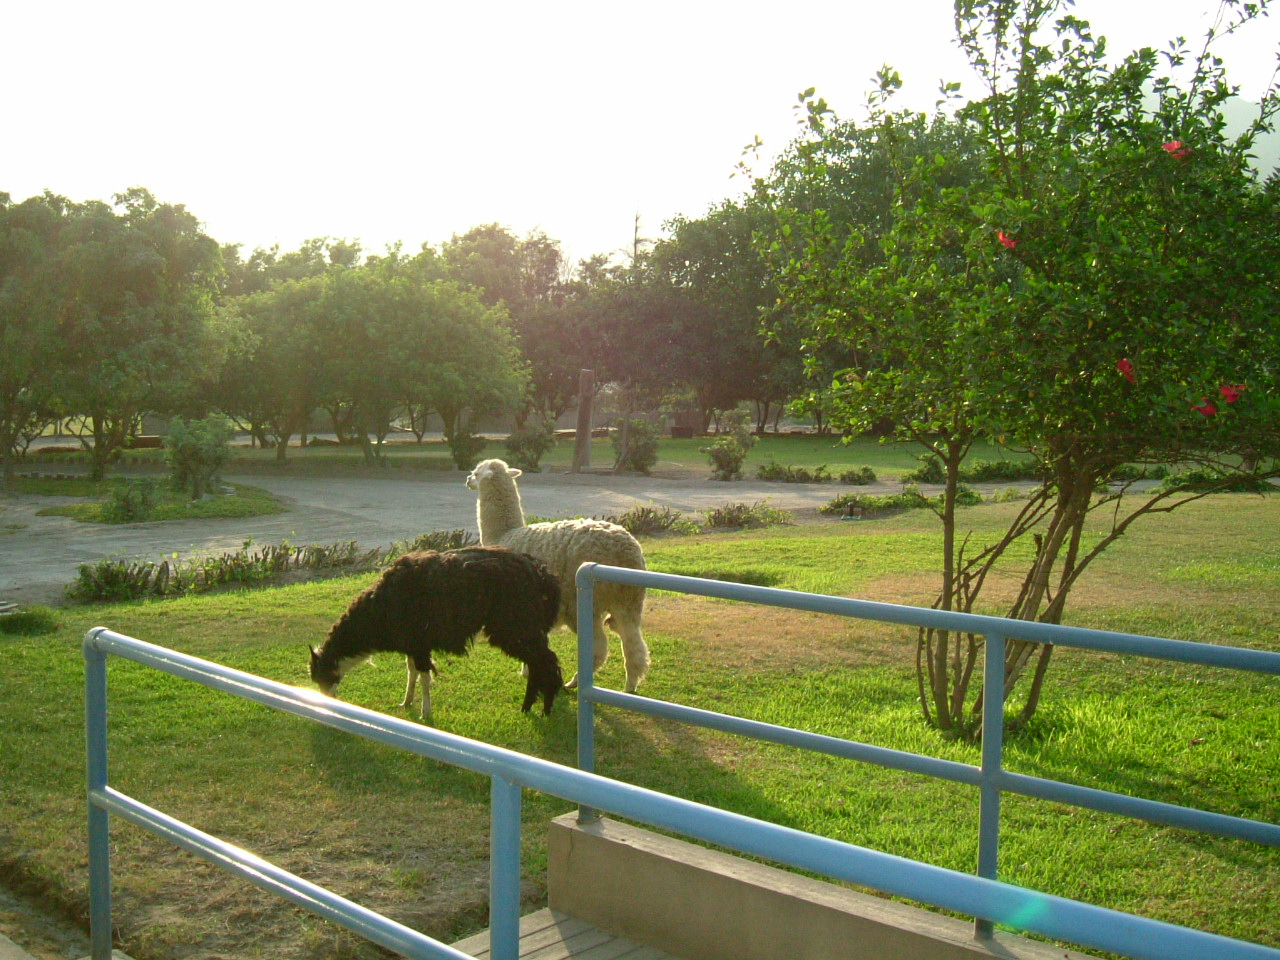
\includegraphics[width=0.6\textwidth]{jicamarca_alpacas}
 \caption[The structure of natural images]{\emph{The structure of natural images.} This digital image of alpacas at Jicamarca is 1280 $\times$ 960 pixels, and at 3 bytes per pixel it would require 3600 KiB of memory to store uncompressed. In its current JPEG compression format, it requires 420 KiB of memory instead. Structure in the image (patterns of color and continuity of edges) is used to reduce the required memory by a factor of about 8.5.}
 \label{fig:jicamarca_alpacas}
\end{figure}%
As a concrete example in the imaging case, consider Figure \ref{fig:jicamarca_alpacas}. Uncompressed, this picture of alpacas at the Jicamarca radar site requires 3600 KiB of memory to store, 1280 $\times$ 960 pixels at 3 bytes per pixel. When compressed in the JPEG format through a discrete cosine transform and by discarding unimportant (small) coefficients to create an exactly sparse representation, this image requires 420 KiB of memory. That's about an 8.5 times savings, representative of the structure inherent in the image and captured in the chosen dictionary.

\subsection{Sparsity in Radar}
\label{intro_radar_sparsity}
Radar signals are not exempt from the sparsity seen in nature. A radar transmits a signal and measures the intensity and phase of any reflections as a function of distance, with Doppler frequency shifts present in the reflection if a target is moving. Reflections from most radar scenes occupy only a small portion of that range-frequency space because the targets themselves are small in number and either spatially limited, have a compact Doppler spectrum from organized movement, or both. Most of the space being observed by the radar does not reflect any signal. Using a dictionary that decomposes signals on a joint range-frequency space captures the natural structure of radar targets and makes the sparsity exploitable.

\subsection{Sparsity in Action}
\label{intro_sparsity_research}
Whether influenced by research into brain physiology or not, the concept of sparsity has come to the fore in many fields of scientific research as a means of speeding, simplifying, or increasing the accuracy of information processing. Often this research falls under the moniker of \emph{compressed sensing}, which exploits sparsity, global measurement, and nonlinear reconstruction to acquire data faster or with higher resolution. Conceptually, since images are often sparse, it does not make sense to measure each pixel individually (as with a regular camera) only to then throw most of that data away to compress it. Instead, compressed sensing takes the approach of directly measuring a compressed representation of the image in order to save time and memory.

Applications of compressed sensing are continually increasing in number. Notable examples that span a variety of fields include the following: the single pixel camera, which uses a filter to randomly mix components of an image and produce a series of mixed-image single pixel readings from which the original image can be reconstructed \autocite{DDT+08}; compressed magnetic resonance imaging, which undersamples the spatial Fourier transform space of the image to speed acquisition and assumes image sparsity to achieve reconstruction \autocite{LDSP08}; and highly-parallel gene screening, which forms overlapping groups of genetic samples from a large set of donors, tests each group in bulk, and assumes rarity of the tracked gene pattern to determine which individual donors have it \autocite{EGB+10, GER12}. Sparsity serves as a useful representation of prior knowledge in all of these and many more applications, so it is no wonder that many fields of research have found success in leveraging sparsity to make important advances.

\section{Contributions}
\label{contributions}
In developing a sparsity-based radar technique for flexible, high-resolution measurement of ionospheric plasmas, this dissertation makes several important contributions:
\begin{itemize}
 \item \emph{A new perspective for radar measurements is espoused in which the radar scene reflectivity is recovered by inverting a mathematical model.}
 \begin{itemize}[]
  \item It is intuitively known that radar signals are sparse in a delay-frequency basis, but traditional approaches are not well-equipped to take advantage of that fact. A discrete radar model that captures signal sparsity is proposed using an image-blurring analogy, and this model is noted to be the adjoint of the standard pulse compression technique that uses a matched filter bank. Thanks to this connection between the two methods, an intuitive interpretation of the inversion technique as an iterative thresholding matched filter is presented.
 \end{itemize}
 \item \emph{A discrete radar model is rigorously derived from the continuous measurement equation for a general target scene.}
 \begin{itemize}[]
  \item The derivation results in an explicit formulation for how the discrete model's reflectivity coefficients represent arbitrary distributed scatterers. Using this expression, it is shown that true target sparsity is reasonably preserved in the discrete representation provided that the number of frequency grid points is high.
 \end{itemize}
 \item \emph{A novel waveform inversion technique is formulated based on finding a sparse representation of the radar scene using the discrete model.}
 \begin{itemize}[]
  \item Recovery of the true solution via $l_1$-norm minimization is proposed based on the theory of compressed sensing. This theory is leveraged to provide theoretical guarantees for the recovery of the true solution provided that the radar pulse waveform produces sufficiently incoherent measurements and that the number of measurements is at least on the order of the solution's sparsity. Waveform inversion is shown to eliminate matched filter sidelobe artifacts and enable higher-resolution solutions.
 \end{itemize}
 \item \emph{The waveform inversion method is implemented using modern convex optimization techniques tailored for efficient computation.}
 \begin{itemize}[]
  \item The focus is on algorithms based on the proximal operator because of their performance, ease of use, and ability to handle large problem dimensions. Since these algorithms are an active area of research, the implementation combines acceleration and adaptive step size enhancements from separate formulations to enable state-of-the-art convergence performance. All computer code is made freely available as open-source software to encourage further development, adoption, and collaboration.
 \end{itemize}
 \item \emph{The real-world flexibility and effectiveness of the inversion technique is demonstrated by the elimination of filtering artifacts from meteor observations made with a variety of standard radar waveforms.}
 \begin{itemize}[]
  \item Successful inversion is shown to depend on the compactness of the peak of the waveform's ambiguity function, while quality of the solution is shown to depend on the fidelity of the transmitted waveform to its idealized model. Increased resolution of the inversion solution is demonstrated but not validated, although the results are promising for future applications.
 \end{itemize}
\end{itemize}

\section{Reader's Guide}
\label{outline}
This dissertation is divided into four parts that build on one another but are relatively self-contained: introduction, radar analysis, waveform inversion, and conclusion. The preceding introduction is intended to familiarize the reader with the primary topics of interest in order to motivate and connect the work as a whole. Part \ref{part_radar_analysis} concerns radar analysis and goes into more detail about how radar measurements are made: Chapter \ref{radar_background} describes current waveform coding and processing techniques and discusses their limitations; Chapter \ref{radar_model} details the derivation and analysis of a mathematical radar model, providing a different way of analyzing radar measurements. The next segment, Part \ref{part_waveform_inversion}, introduces a waveform inversion method that combines the radar model with prior information of sparsity: Chapter \ref{sparsity_background} describes the theory of compressed sensing and related methods of convex optimization; Chapter \ref{waveform_inversion} details the implementation of the waveform inversion technique, including algorithmic advances; and Chapter \ref{experimental_results} provides experimental results using the Jicamarca radar to test waveform inversion and compare the effect of different waveforms. Finally, Part \ref{part_conclusion} contains the concluding chapter, which discusses the benefits provided by the new techniques and highlights areas for future research. One appendix is included, Appendix \ref{reflectivity_coefficients}, which details the simplification of the reflectivity coefficient expression derived in Chapter \ref{radar_model} as part of the radar model.

%The other two appendices cover techniques that are especially helpful for processing meteor data: Appendix \ref{clustering} describes a clustering approach that enables automatic detection and classification of radar signals; and Appendix \ref{super_resolution} describes the interpolated matched filter method used for super-resolution of range and range-rate estimates and analyzes its statistical accuracy via simulation.